\chapter{Information Visualization}
\label{chap:InfoVis}

Information visualization is the science of representing abstract information as interactive graphics to present and analyze it more efficiently.
These two goals of presenting and analyzing abstract information in a visual form are built on the properties of human visual perception, which include the rapid scanning, recognition and recollection of visual information as well as the automatic detection of patterns in it.
In contrast to textual representations of data, the processing of well-designed visualizations requires much less cognitive effort because it leverages features of the human visual processing system.
One of these features is preattentive processing, which means that certain visual attributes can be processed very quickly and without any conscious effort \parencite{PreattentiveProcessing}.

In addition to visuals being easier to assimilate by humans, a purely textual and statistical view on data can also lead to erroneous assumptions as demonstrated by \cite{AnscombesQuartet} in the infamous visualization of four completely different datasets which have identical summary statistics, called Anscombe's Quartet.
An observer trying to understand these sets of data purely from their statistics would mistakenly deem them to be identical.
Their inequality will only become obvious after carefully examining and comparing the individual entries in the datasets themselves.
This is a tedious and error-prone task when not aided by visual representations like Figure \ref{fig:AnscombesQuartet}.
Even though Anscombe's Quartet is very likely the most famous example to demonstrate this characteristic, it is certainly not the only set of datasets which possesses it, as has been shown by \cite{GenDataIdenticalStatisticsDissimilarGraphics}.

\begin{figure}[tp]
\centering
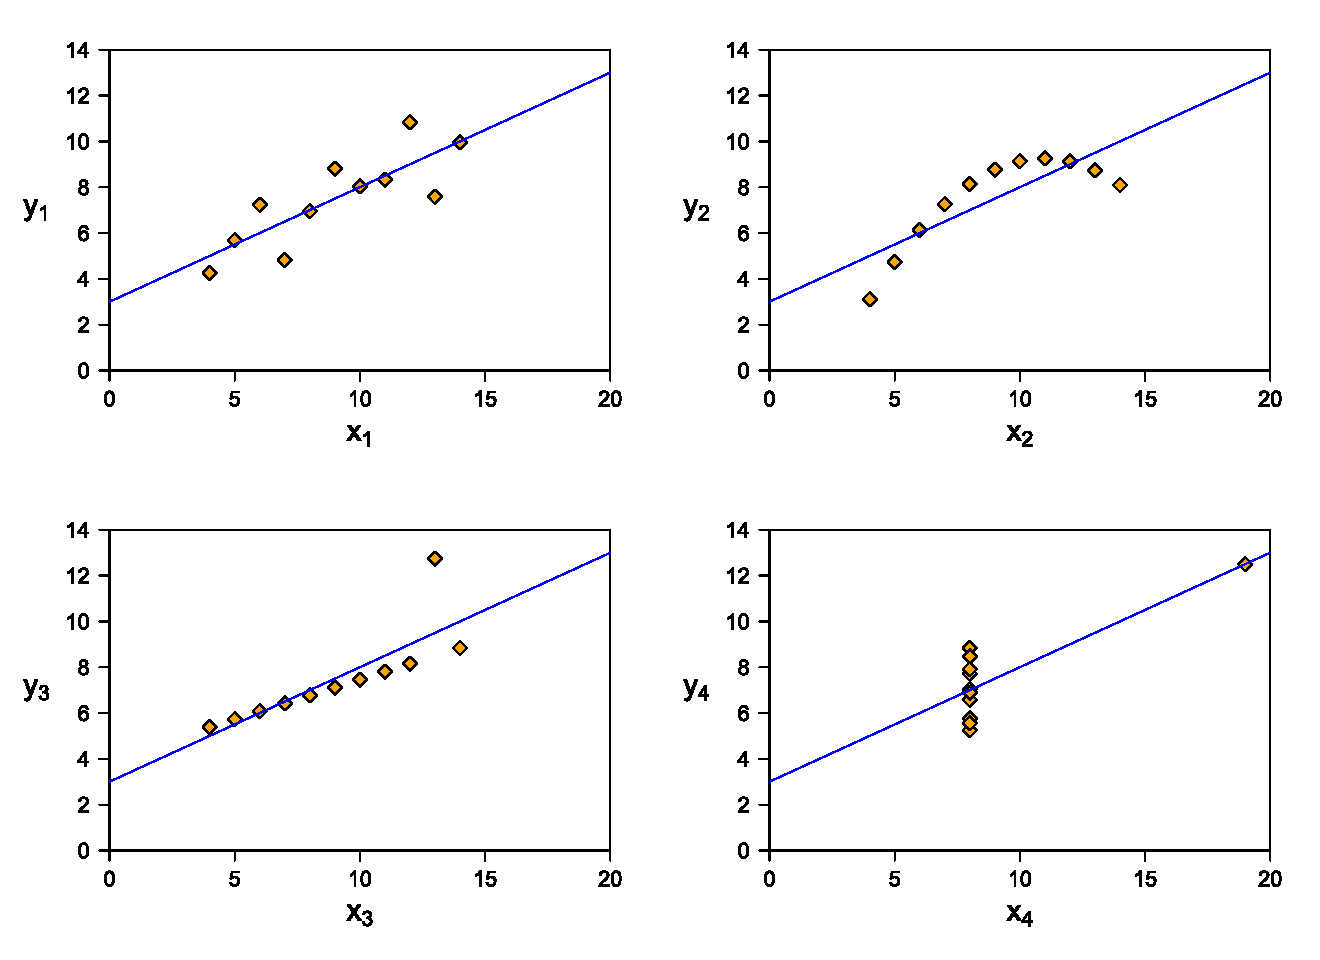
\includegraphics[keepaspectratio,width=\linewidth,height=\fullh / 3]{diagrams/anscombe.pdf}
\caption[Anscombe's Quartet]{
  Anscombe's Quartet consists of four distinct sets of data which share identical summary statistics.
  The difference between these datasets is only obvious by carefully examining the textual data or by plotting it.
  \imgcredit{Image extracted from \cite{IVISCourseNotes}. Used with kind permission by Keith Andrews.}
}
\label{fig:AnscombesQuartet}
\end{figure}

This thesis adheres to the separation of the field defined by \cite{IVISCourseNotes}. 
It is stated that the field of visualization is segmented into the three main subfields of information visualization, geographic visualization and scientific visualization. 
Furthermore, the often used term "data visualization" is defined as the intersection of geographic visualization and information visualization.

\begin{enumerate}
\item Information Visualization: Deals with abstract data, which has no inherent presentation and for which a suitable type of visualization has to be chosen.
\item Geographic Visualization: Deals with map-based data which has an inherent spatial dimension. 
\item Scientific Visualization: Deals with object-related data which has inherent presentation, which is usually related to the object's real-world representation.
\end{enumerate}

Visualizations presented in an interactive medium do not merely consist of visual representations.
It is equally important to provide means for interacting with these representations to analyze more complex datasets.
Without interactions, a visualization is just a static image and has only very limited use when dealing with large and multidimensional data.
Even though the majority of the attention in the field of information visualization has been put on the presentational aspect of visualizations, a lot of research has also been conducted on their interactive aspects.
Many taxonomies have been formulated with the goal of defining the design space of interactions to support analytic reasoning, but they vary greatly depending on the concepts they are focusing on.
Some taxonomies have been defined on the concept of low-level interaction techniques \parencite{TheEyesHaveIt,GrammarOfGraphics}, providing a very system-centric view on interaction. 
Other taxonomies focus on user tasks \parencite{LowLevelComponentsOfAnalyticActivity} which are not necessarily strongly related to interacting with visualizations.
\cite{RoleOfInteractionInInformationVisualization} aims to provide a view in between the purely system-centric and purely user-centric extremes by defining a taxonomy based on user intent.
The categories of this taxonomy are listed in Table \ref{tab:UserIntentCategories}
They form a good framework for the discussion of interactivity in the context of information visualization.

\begin{table}[tp]
\tablestretch
\rowcolors{2}{}{tablerowcolour}
\centering
\begin{tabularx}{\linewidth}{>{\kern-\tabcolsep}lXX<{\kern-\tabcolsep}}
\toprule
Category & Description & Examples \\
\midrule
Select & Mark items as interesting. & \\
Explore & Show different items. & Panning, direct-walk \\
Reconfigure & Show a different arrangement. & Dimension configuration, position adjustments \\
Encode & Show a different representation. & Change chart type, orientation, colors, shapes, ... \\
Abstract/Elaborate & Show more or less detail. & Details-on-demand (drill-down, sunburst, tooltips, zooming) \\
Filter & Show items based on conditions. & Dynamic query controls \\
Connect & Show related items. & Highlight connected items, highlight item in different representations \\
\bottomrule
\end{tabularx}
\caption[Categories of Interaction Based on User Intent]{
  This table shows the categories of interacting with visualizations based on user intent.
  \imgcredit{Table adapted from \cite{RoleOfInteractionInInformationVisualization}}
}
\label{tab:UserIntentCategories}
\end{table}



\section{History of Information Visualization}

The history of Information Visualization goes back a long time with one of the earliest examples dating back to the 10th century, when an unknown astronomer created a chart about the movement of prominent planets \parencite{CommentariiInSomniumScipionis}, shown in Figure \ref{fig:PlanetaryMovements}.
Other noteworthy early visualizations include the first occurrence of the principle \cite{VisualDisplayOfQuantitativeInformation} later coined "small multiples" in a 1626 chart demonstrating sunspot changes (Figure \ref{fig:SunspotChanges}) by \cite{RosaUrsina} and a 1644 chart displaying longitudinal distance determinations between Toledo and Rome (Figure \ref{fig:RomeToledoLongitude}) by Michael Florent van Langren.

\begin{figure}[tp]
\centering
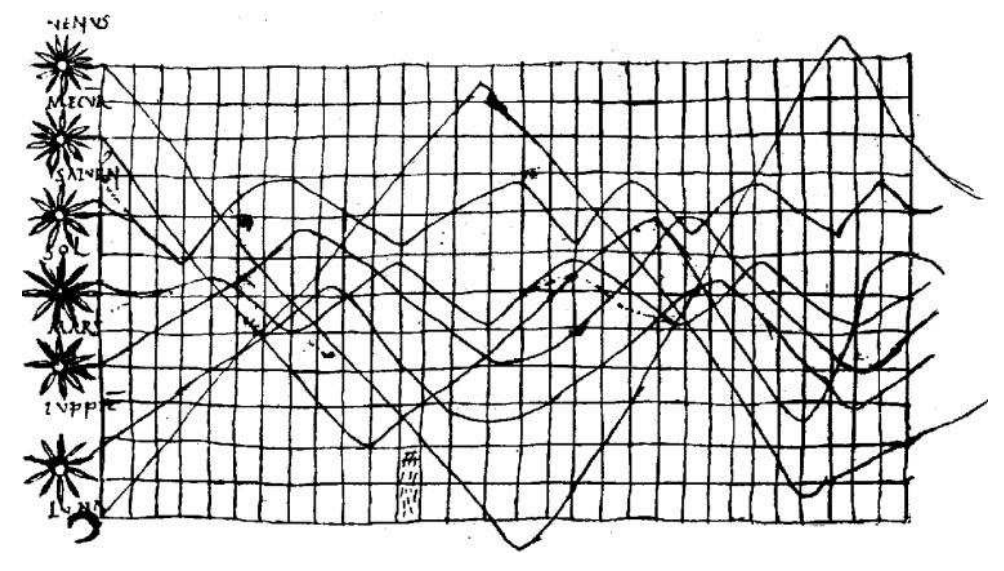
\includegraphics[keepaspectratio,width=\linewidth,height=\fullh / 3]{images/planetary-movements.png}
\caption[Chart of Planetary Movements from the Tenth Century]{
  A chart created by an unknown astronomer in the tenth century depicting the movements of seven prominent planets.
  \imgcredit{Image extracted from \cite{BriefHistoryOfDataVis}. Original appearance in \cite{CommentariiInSomniumScipionis}.}
}
\label{fig:PlanetaryMovements}
\end{figure}

\begin{figure}[tp]
\centering
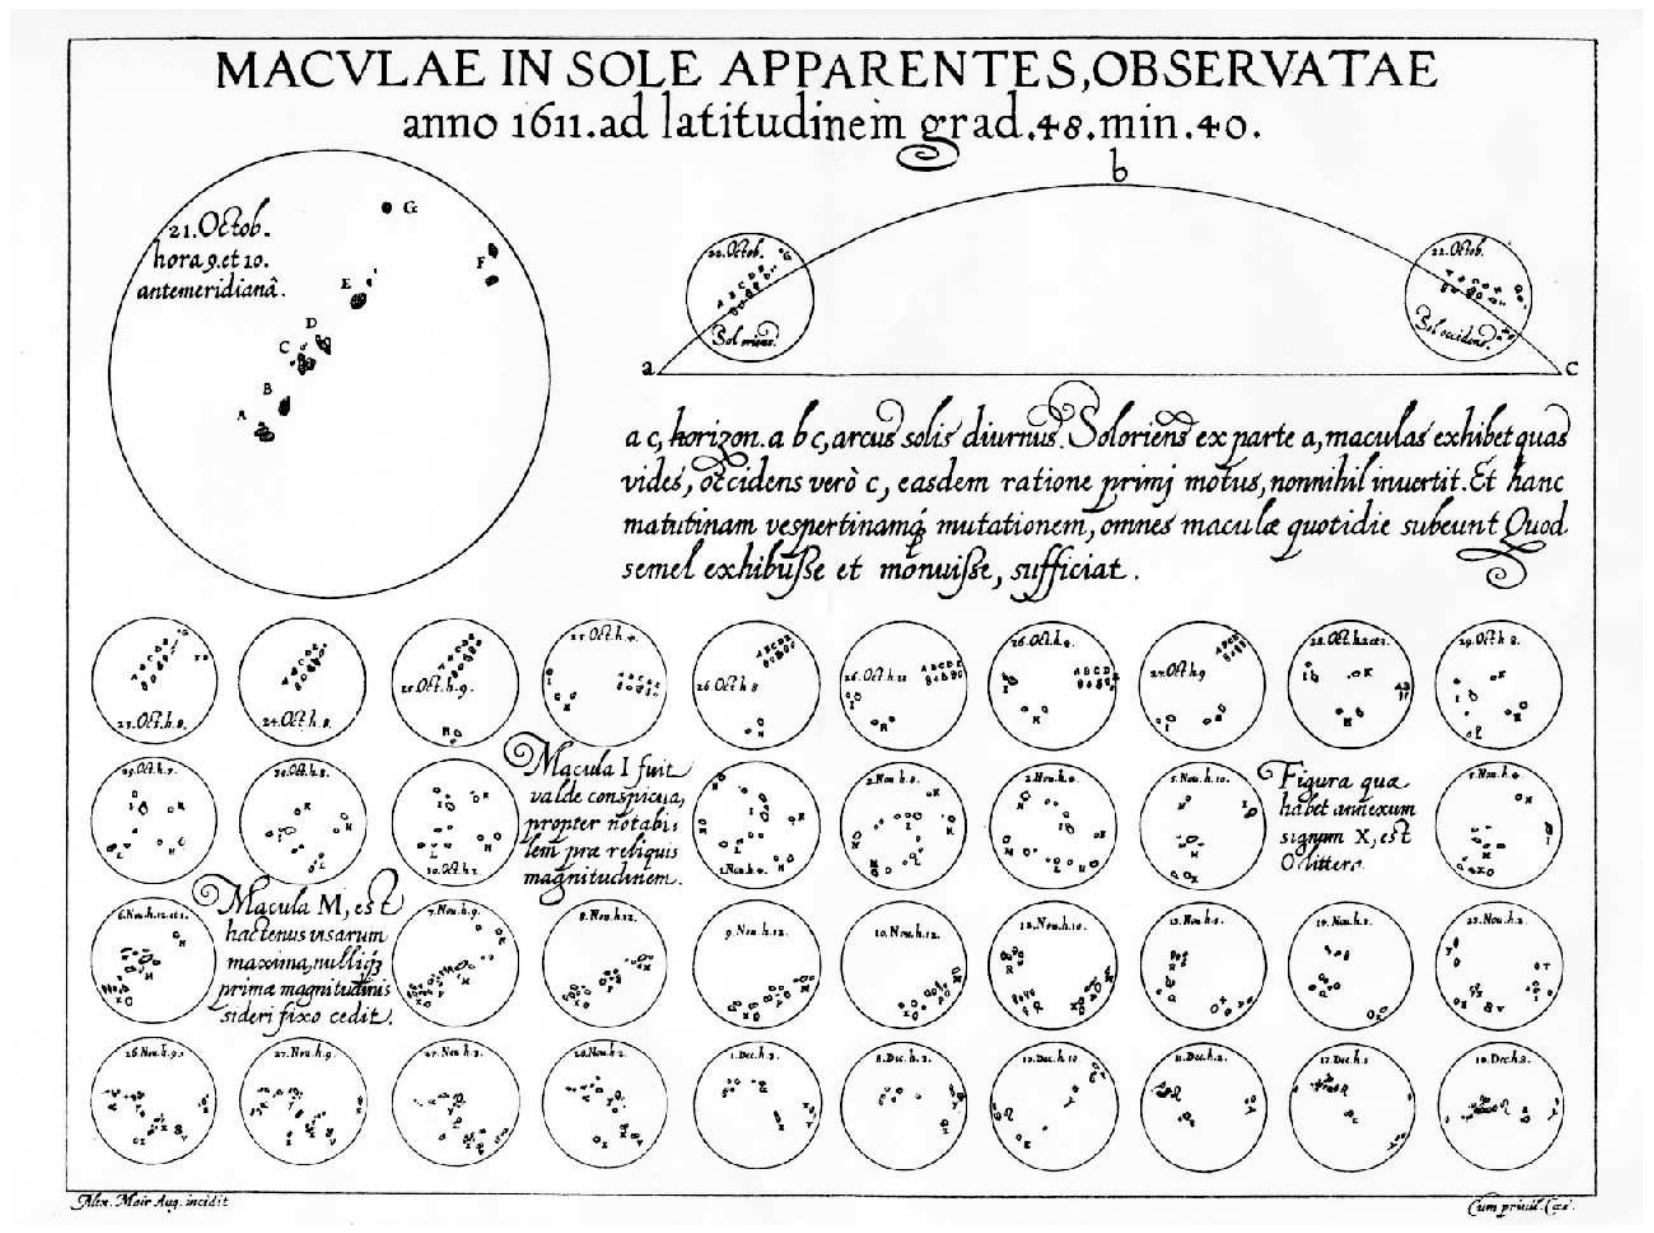
\includegraphics[keepaspectratio,width=\linewidth,height=\fullh / 3]{images/sunspot-changes.png}
\caption[Chart of Changes in Sunspots from 1626]{
  This chart shows the observed changes in sunspots based on recordings of two months of data from 1611.
  It is the first occurrence of the principle later called "small multiples" by \cite{VisualDisplayOfQuantitativeInformation}.
  \imgcredit{Image extracted from \cite{BriefHistoryOfDataVis}.Original appearance in \cite{RosaUrsina}.}
}
\label{fig:SunspotChanges}
\end{figure}

\begin{figure}[tp]
\centering
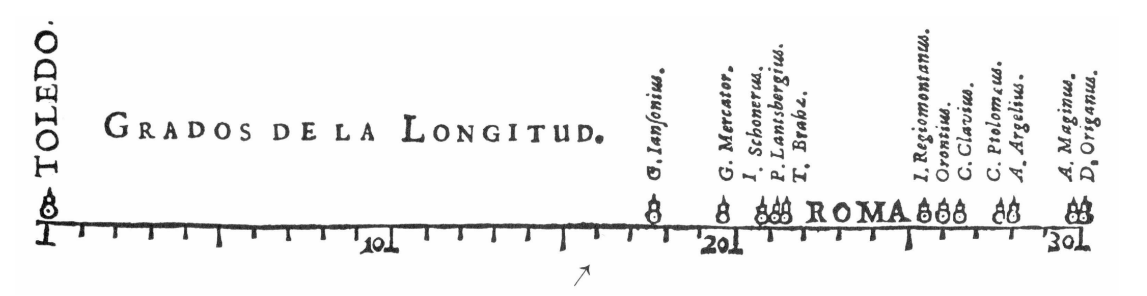
\includegraphics[keepaspectratio,width=\linewidth,height=\fullh / 3]{images/rome-toledo-longitude.png}
\caption[Chart of Longitudinal Distance Determinations Between Toledo and Rome From 1644]{
  This chart compares the twelve known estimates in longitudinal distance between Rome and Toledo by various astronomers.
  The correct distance is marked by the arrow beneath.
  It is considered to be the first visual representation of statistical data.
  \imgcredit{Image extracted from \cite{BriefHistoryOfDataVis}. Original appearance in \cite{VisualExplanations}.}
}
\label{fig:RomeToledoLongitude}
\end{figure}

William Playfair (1759 - 1823) is by many considered to be one of the forefathers of modern visualizations.
His published works contain the first occurrences of many graphical forms still widely used today.
In one of his earlier works \parencite{CommercialAndPoliticalAtlas} he introduced the concepts of line (Figure \ref{fig:PlayfairLineChart}), bar (Figure \ref{fig:PlayfairBarChart}) and area charts (Figure \ref{fig:PlayfairAreaChart}) to communicate economic factors of England during the eighteenth century.
In a related later work \parencite{StatisticalBreviary} he uses the first ever published pie and circle charts to show and compare the resources of states and kingdoms in Europe.
The charts he created are very similar to modern ones because they already contain major concepts found in today's visualizations, such as labeled axes, grids, titles and color-based categorization.

\begin{figure}[tp]
\centering
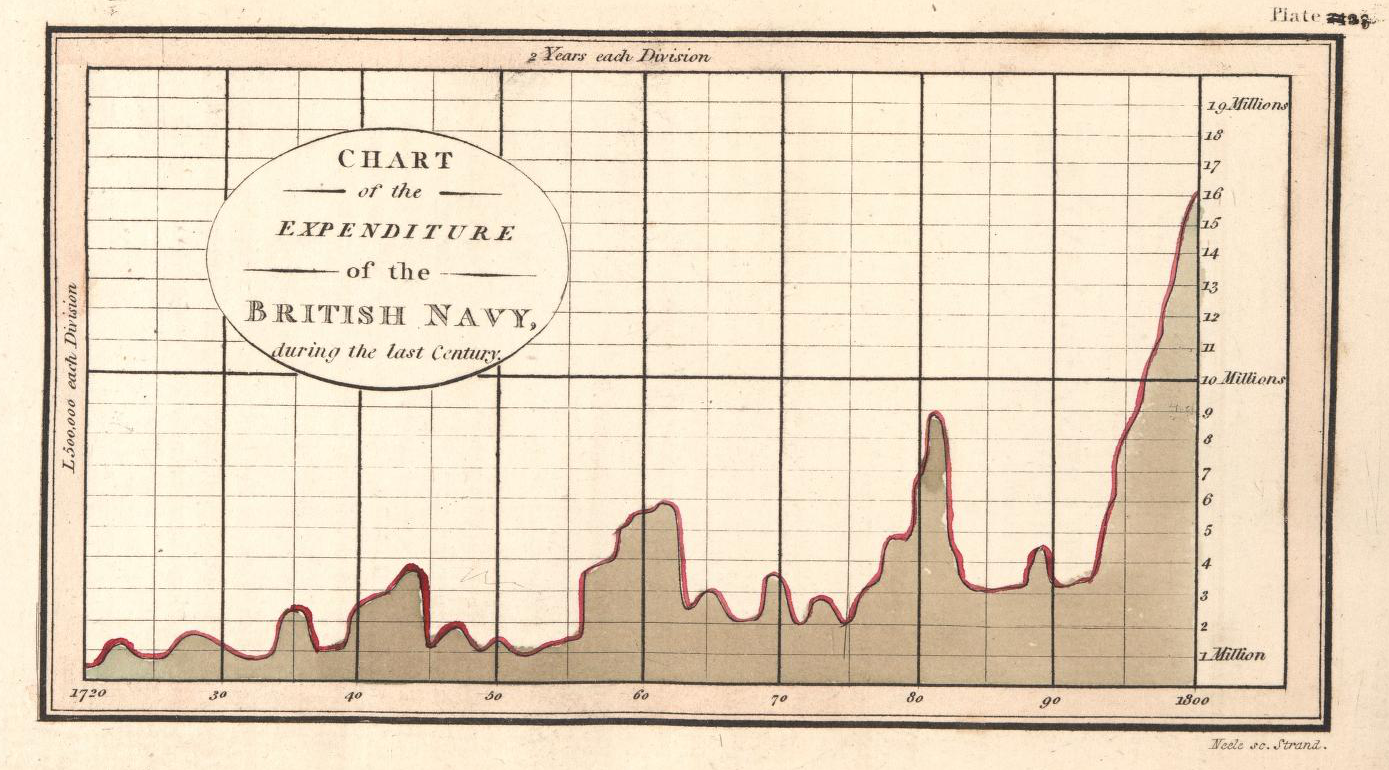
\includegraphics[keepaspectratio,width=\linewidth,height=\fullh / 3]{images/playfair-line-chart.png}
\caption[Line Chart by William Playfair From 1786]{
  This chart shows the expenditure of the British navy during the eighteenth century as a line chart.
  It was published in 1786 and is considered to be one of the first occurrences of a line chart containing most components found in modern visualizations.
  \imgcredit{Image extracted from Schoenberg Center for Electronic Text and Image (SCETI). Used under the terms of Creative Commons CC BY 2.5.}
}
\label{fig:PlayfairLineChart}
\end{figure}

\begin{figure}[tp]
\centering
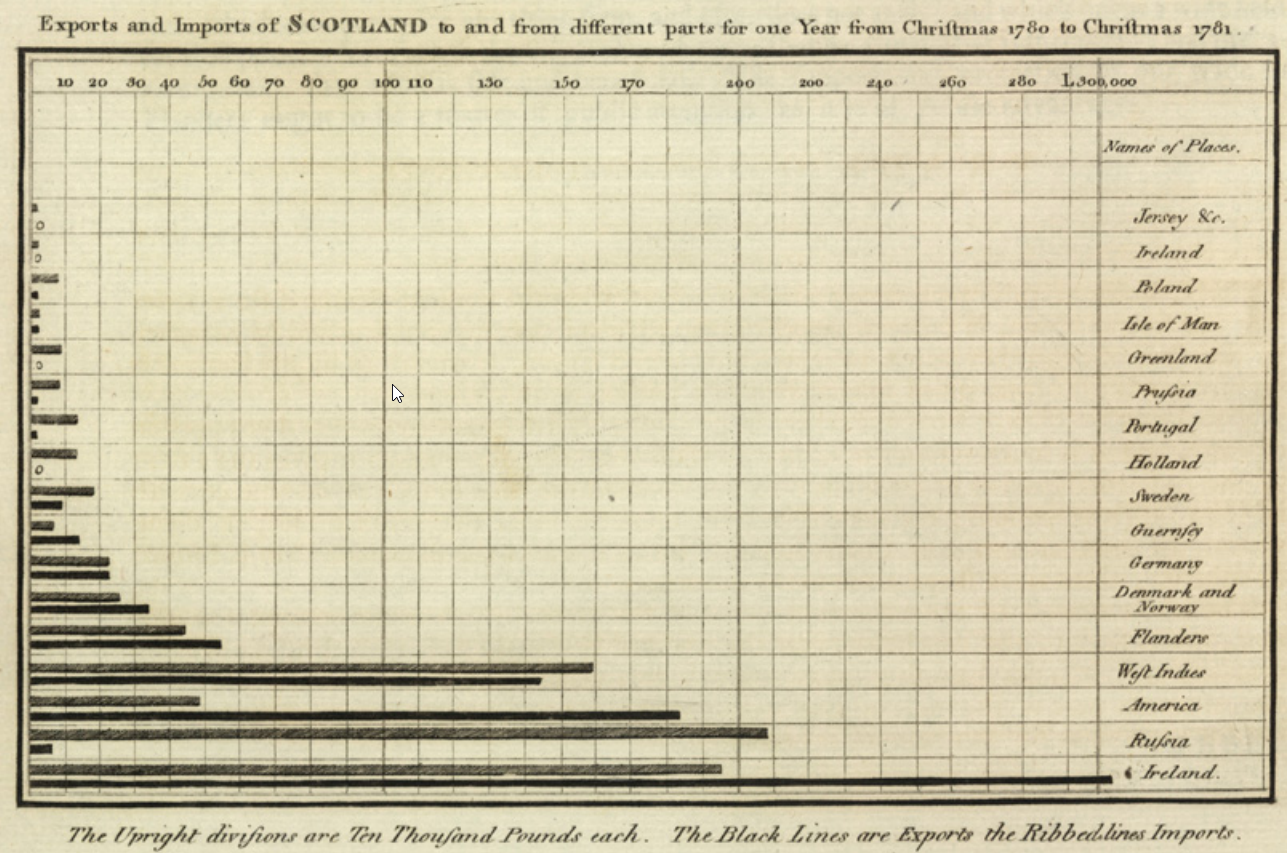
\includegraphics[keepaspectratio,width=\linewidth,height=\fullh / 3]{images/playfair-bar-chart.png}
\caption[Bar Chart by William Playfair from 1786]{
  This chart shows England's exports and imports from and to Scotland in 1781 visualized as a bar chart.
  It was published in 1786 and is considered to be one of the first occurrences of a bar chart containing most components found in modern visualizations.
  \imgcredit{Image extracted from Schoenberg Center for Electronic Text and Image (SCETI). Used under the terms of Creative Commons CC BY 2.5.}
}
\label{fig:PlayfairBarChart}
\end{figure}

\begin{figure}[tp]
\centering
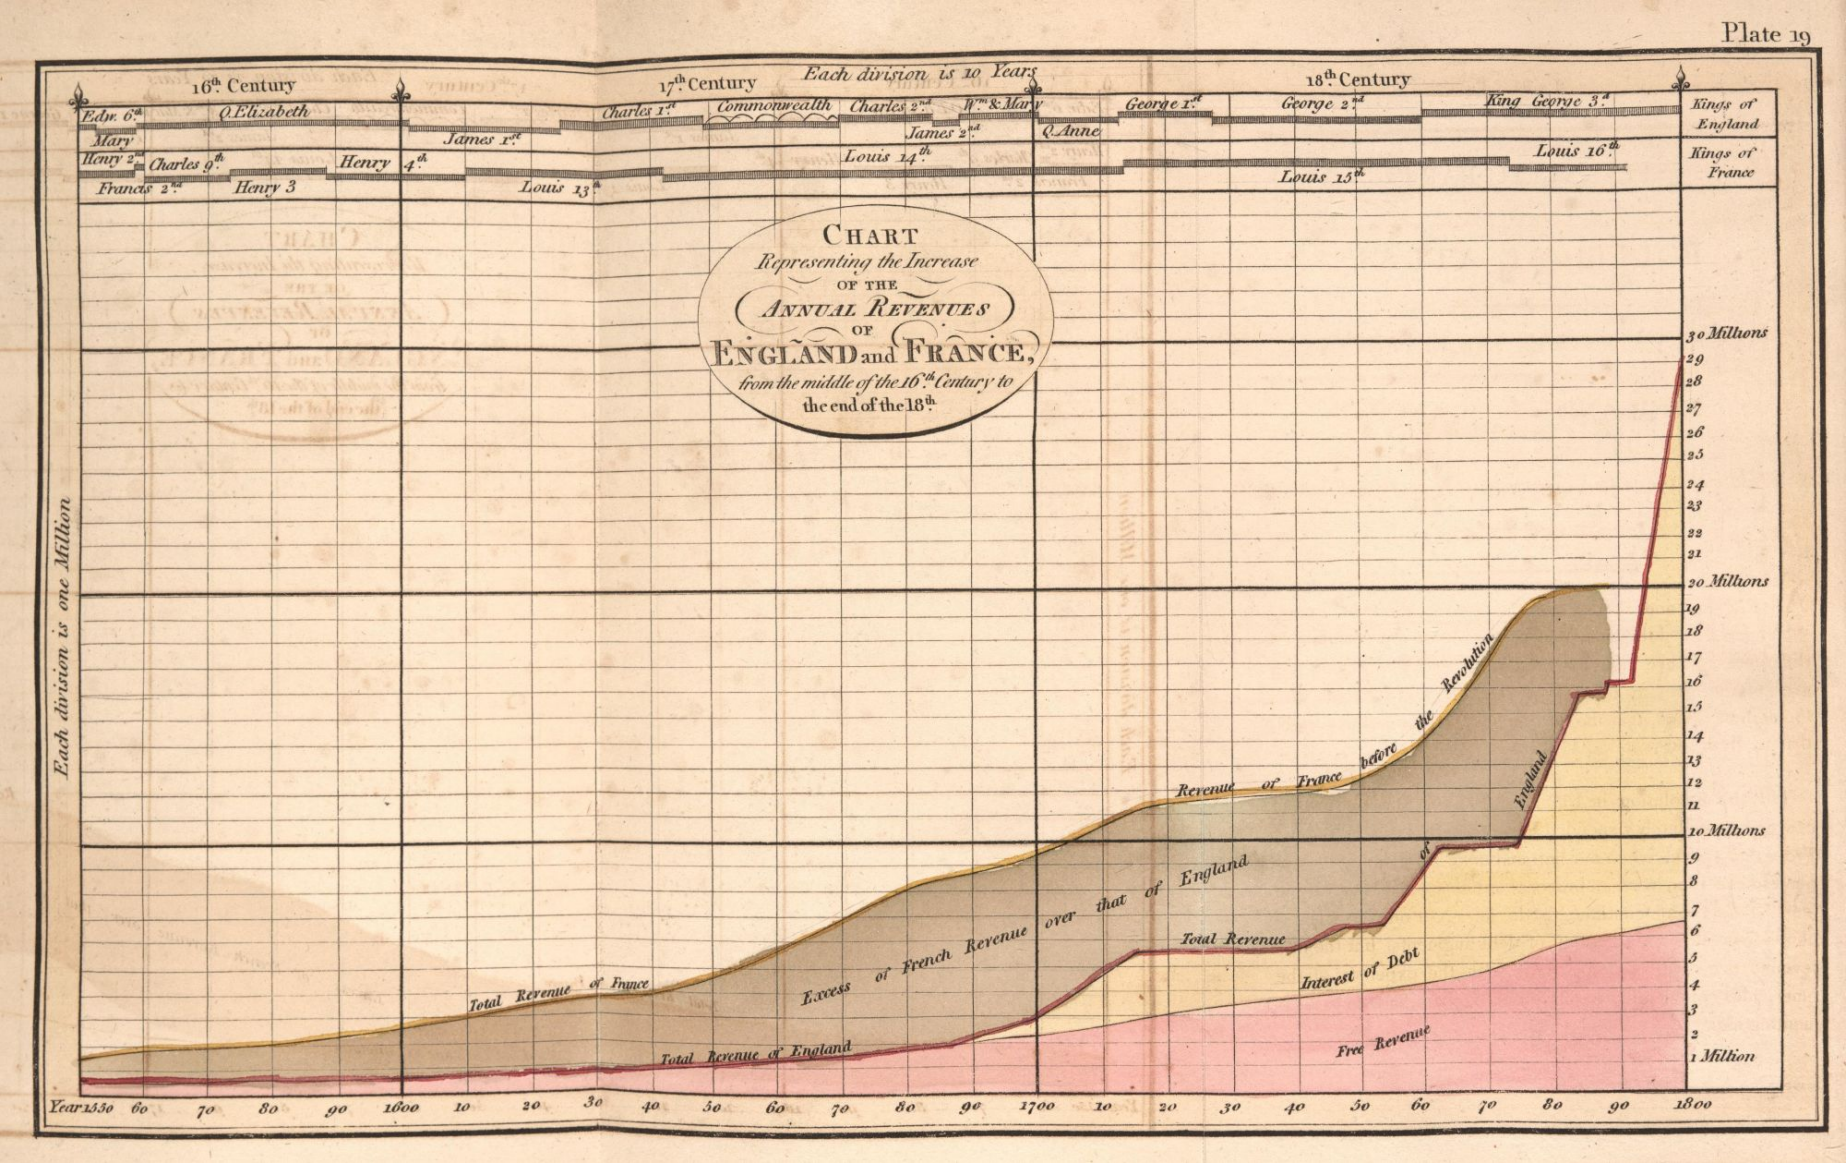
\includegraphics[keepaspectratio,width=\linewidth,height=\fullh / 3]{images/playfair-area-chart.png}
\caption[Area Chart by William Playfair from 1786]{
  This chart shows the annual revenues of England and France between 1550 and 1800 visualized as an area chart.
  It was published in 1786 and is considered to be one of the first occurrences of an area chart containing most components found in modern visualizations.
  \imgcredit{Image extracted from Schoenberg Center for Electronic Text and Image (SCETI). Used under the terms of Creative Commons CC BY 2.5.}
}
\label{fig:PlayfairAreaChart}
\end{figure}

The dot map created by \cite{ModeOfCommunicationOfCholera} in 1855 to trace cholera outbreaks in London (Figure \ref{fig:CholeraDotMap}) is undoubtedly one of the most famous and influential visualizations in history.
Even though it is not directly an information visualization but rather a geographic one, it has been included here because of its historic relevance.
This iconic dot map was used to identify a cluster of cholera-related deaths near a contaminated water pump on Broad Street, leading to the recognition of cholera as a waterborne disease.

\begin{figure}[tp]
\centering
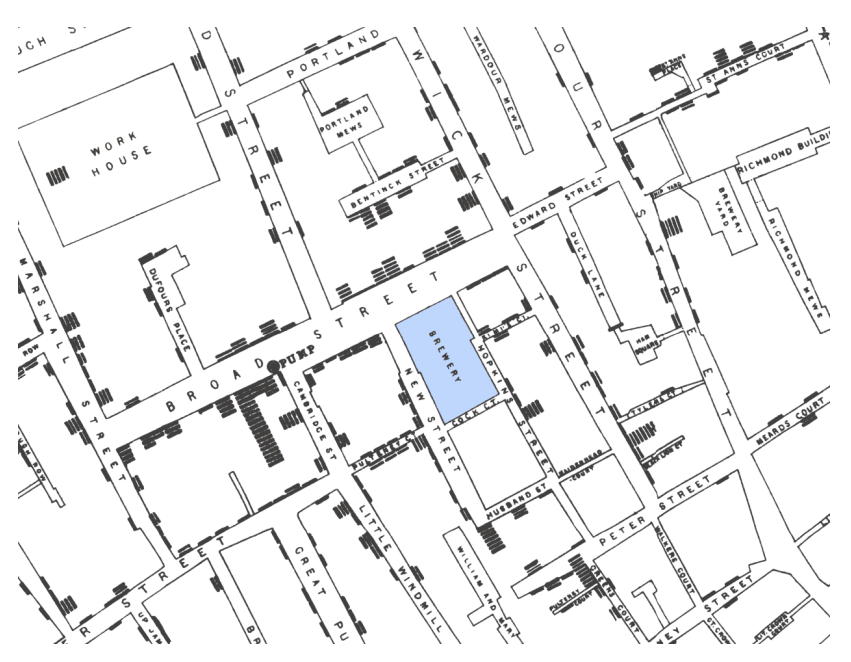
\includegraphics[keepaspectratio,width=\linewidth,height=\fullh / 3]{images/cholera-dot-map.png}
\caption[Dot Map Plotting Cholera Deaths in London From 1855]{
  This iconic chart was created by Dr. John Snow in 1855 to identify a clustering of cholera-related deaths near Broad Street in London.
  It was used to identify a contaminated water pump and to illustrate the waterborne nature of the disease.
  Since the data is map-based, this chart is an example of a geographic visualization rather than an information visualization.
  \imgcredit{Image extracted from \cite{IVISCourseNotes}. Original appearance in \cite{ModeOfCommunicationOfCholera}.}
}
\label{fig:CholeraDotMap}
\end{figure}

It would go amiss not to mention Florence Nightingale (1820 - 1910) \parencite{FlorenceNightingale} when talking about the history of information visualization.
She was a British statistician, social reformer, founder of modern nursing and might be the first person who used visualizations to persuade others of a need for change.
During her service as a superintendent of nurses in the Crimean War, she realized that a large share of deaths in hospitals resulted from preventable diseases which originated in poor sanitary conditions.
One of her contributions to the field of information visualization was the creation of a new type of diagram, called a rose or polar-area chart.
She used these charts to communicate data she collected on the mortality of soldiers during the war and to grab the attention of politicians and the public.
One of these charts can be seen in Figure \ref{fig:NightingalePolarAreaChart}.

\begin{figure}[tp]
\centering
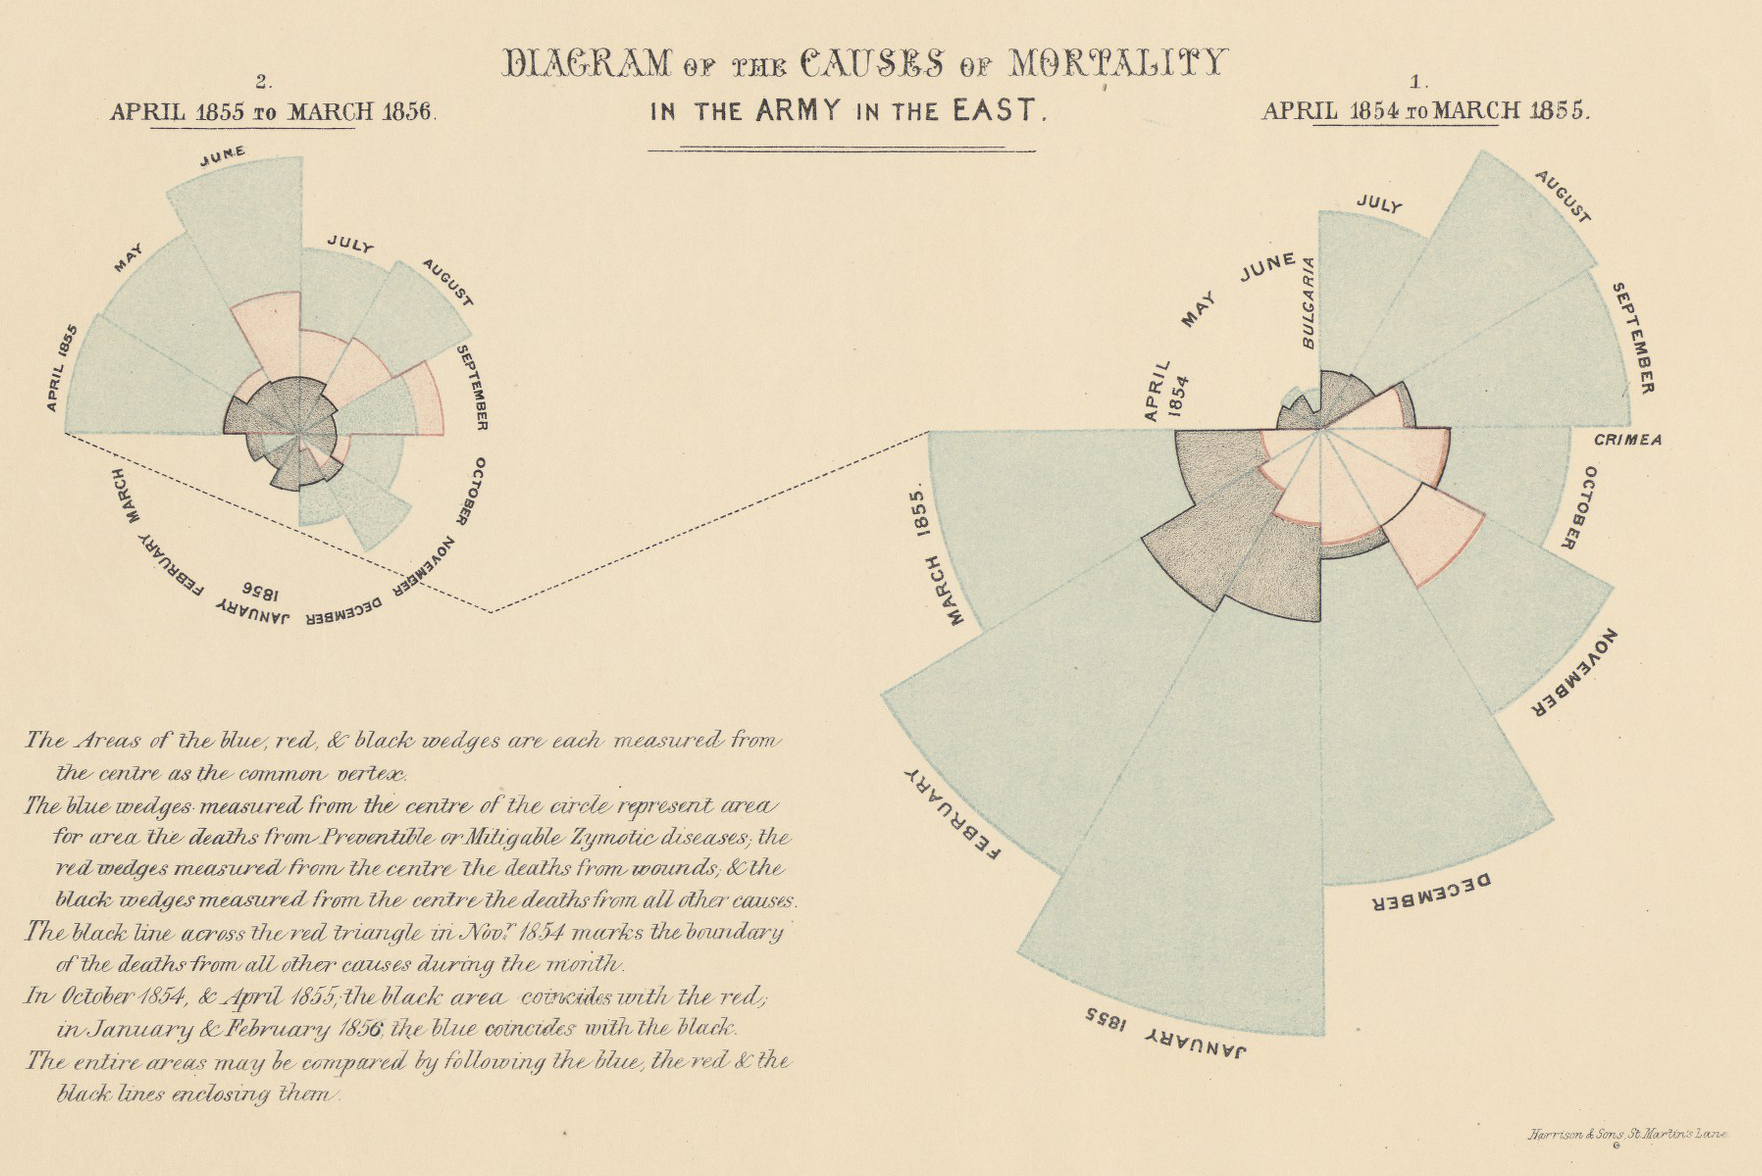
\includegraphics[keepaspectratio,width=\linewidth,height=\fullh / 3]{images/nightingale.png}
\caption[Polar-Area Chart by Florence Nightingale From 1859]{
  This is one of the polar-area charts that Florence Nightingale created in 1859 to convince people of a need for more sanitary conditions in hospitals.
  It visualizes the causes of mortality for soldiers during the Crimean War and demonstrates that a large percentage of patients died from preventable diseases which are linked to unsanitary environments.
  \imgcredit{Image extracted from Harvard Library. Used under the terms of Creative Commons Attribution 4.0.}
}
\label{fig:NightingalePolarAreaChart}
\end{figure}

Modern visualizations benefit from the interactive nature of the devices used to consume them.
They are allowed to be a lot more complex than static visualizations because various interaction techniques enable users to navigate large amounts of data and make sense of it.
High-D by the company Macrofocus \parencite{HighD} has been chosen as a representative example of such visual analytics tools, and a screenshot of its interface during the analysis of a sample dataset can be seen in Figure \ref{fig:HighD}.

\begin{figure}[tp]
\centering
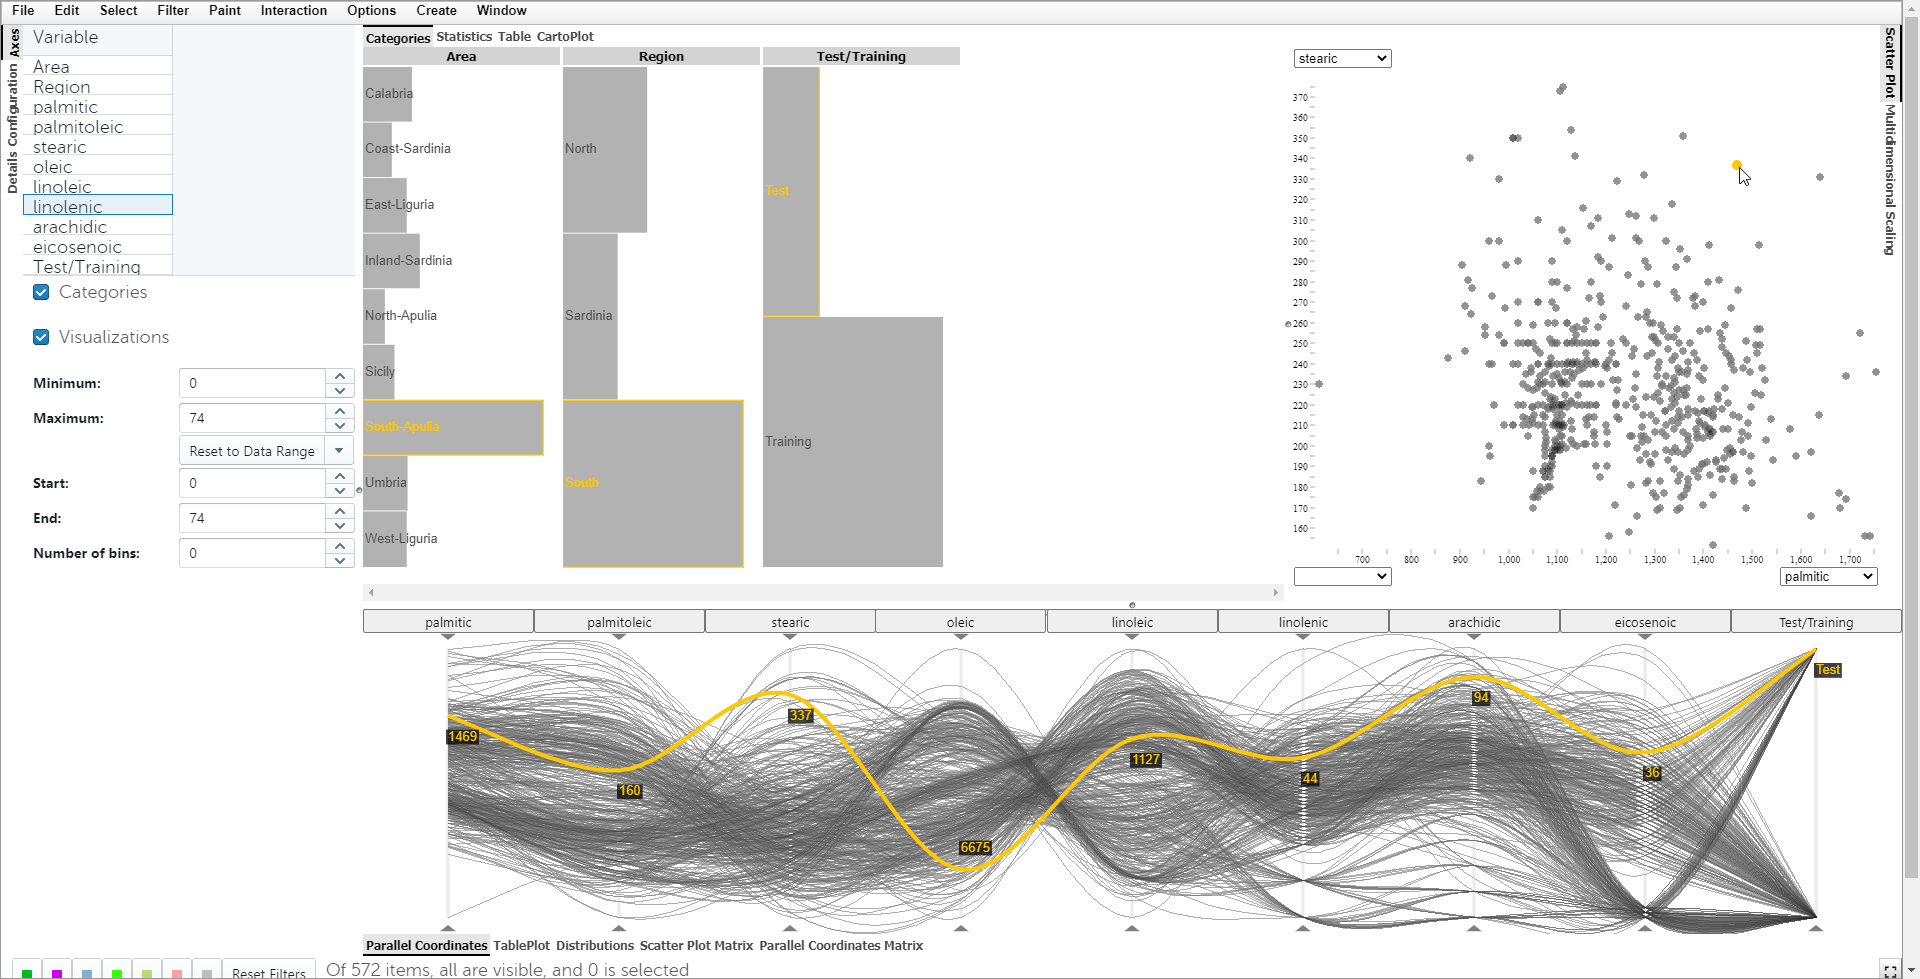
\includegraphics[keepaspectratio,width=\linewidth,height=\fullh / 3]{images/high-d.png}
\caption[Screenshot of High-D]{
  High-D from the company Macrofocus is a visual analytics tool specialized in analyzing multidimensional data.
  \imgcredit{Screenshot of \cite{HighD} taken by the author of this work.} \TODO{How to cite this? Copyright?}
}
\label{fig:HighD}
\end{figure}

It is out of the scope of this work to provide a full account over the long and eventful history of information visualization.
This section only provides a brief and very selective view on the topic and much more comprehensive works exist which go significantly deeper into details of the various actors and the intricate influences they had on each other.
Recommendable sources for further reading on the history of visualization include \cite{BriefHistoryOfDataVis}, \cite{HistoryOfDataVisAndGraphicCommunication} and \cite{HistoryOfInformationGraphics}.

\section{Information Visualization Libraries for the Web}

There are many web-based libraries which simplify the rendering of interactive visualizations.
The approaches used to create and update visualization can be vastly different between libraries.
D3 is a low-level library which enables data-driven transformations of documents, Vega and Vega-Lite provide a declarative grammar which enables the expression of visual and interactive characteristics of visualizations, and template-based visualization libraries provide a template-based interface which can easily be configured.
These libraries and some of their characteristics will be summarized in the following sections.

\subsection{Data-Driven Documents (D3)}

D3 \parencite{D3} is a free and open-source document manipulation library built in JavaScript.
It is maintained by an active GitHub community and its core maintainer Mike Bostock who is also the creator of Observable \parencite{Observable} and the deprecated Protovis visualization library \parencite{Protovis}.

D3 enables data-driven document transformations which allows developers to describe their documents as functions of data.
As an example, developers can define transformations which receive a dataset and transform it into a basic HTML table or into a more sophisticated visualization as an SVG chart.
This focus on explicitly defining transformations is better suited for dynamic visualizations because developers have complete control over the creation, modification and removal of elements.
It also sets D3 apart from other visualization libraries where developers usually define the desired state of a representation using a declarative domain specific language.

In contrast to other visualization libraries, D3 contains no proprietary visual primitives and relies on well established web standards like HTML, SVG and CSS to provide visual representations.
This yields a lot of flexibility because developers work directly with web standards which are implemented by their browsers and do not need to wait for D3 to implement support for new features as standards evolve.
If developers chose to switch to a different library, the knowledge of web standards they gained during their work with D3 might be applicable in their future work.
The reliance on web standards also makes it possible to use debugging tools which are already natively implemented in browsers.

Other important aspects of D3's design include immediate evaluation, the principle of parsimony, and support for method chaining.
Immediately evaluating functions means that operations, such as modifying attributes, are applied instantaneously at the time of calling the respective functions.
This achieves a reduction in internal complexity by handing it over to invoking code and avoids common errors related to missing state changes when state is being modified multiple times between rendering.
The principle of parsimony, also referred to as Occam's razor, is a problem-solving principle which stems from the field of philosophy \parencite{PrincipleOfParsimony}.
It is frequently paraphrased as "entities should not be multiplied beyond necessity" and when applied to API design it means that superfluous functions in an API should be avoided.
As an example, the background color of a circle element can already be set with the generic \lstinline{Selection.attr} method to set the \attrname{background-color} attribute of all elements in a Selection.
Adding an additional \lstinline{backgroundColor} method would violate the principle of parsimony.
Method chaining is a popular syntax which allows functions to be chained after one another to avoid having to store intermediate results into variables which would otherwise not be needed.
It is implemented in D3 by returning the \lstinline{Selection} on which a modifying method is called as a result of that method.
Methods which insert new elements into the DOM, such as \lstinline{Selection.append} and \lstinline{Selection.insert}, return a Selection of the newly added elements instead to enable the creation of nested structures.
This method chaining syntax is further improved by the \lstinline{Selection.call} method which invokes a callback receiving the current Selection as a parameter and returns the original Selection to further chain methods on it after the callback has been executed.
The \lstinline{Selection.call} method enables the creation of complex method chaining structures and is widely used by developers.
A simple example of method chaining in D3 and the application of the \lstinline{Selection.call} method can be seen in Figure \ref{list:D3MethodChaining}.

\begin{samepage}
\lstinputlisting[%
  float=tp,
  aboveskip=\floatsep,
  belowskip=\floatsep,
  xleftmargin=0cm,              % no extra margins for floats
  xrightmargin=0cm,             % no extra margins for floats
  %
  language=JavaScript,
  basicstyle=\footnotesize\ttfamily,
  frame=shadowbox,
  numbers=left,
  label=list:D3MethodChaining,
  caption={[D3 Method Chaining] 
    A simple example of method chaining in D3 which creates an \elname{h1} and \elname{p} element inside a \elname{body}.
  },
]{listings/d3-method-chaining.js}
\end{samepage}

Selections have already been mentioned in the previous paragraphs.
They are the atomic building blocks of D3 which are used to access almost any functionality.
Selections are created using the \lstinline{d3.select} or \lstinline{d3.selectAll} methods.
These methods are built on the DOM Selectors API, namely the \lstinline{querySelector} and \lstinline{querySelectorAll} methods, which allow the selection of elements via CSS selectors (see Section \ref{sec:CSS}), and which consequentially allow the \lstinline{d3.select} and \lstinline{d3.selectAll} methods to either create a Selection containing a single element matching the provided selector or to create one which contains multiple elements matching it.
A Selection acts as a wrapper container around these selected elements, and it provides methods to perform frequently performed DOM operations on them.
Among others, the element operations provided by a Selection include the setting and getting of: Attributes using the \lstinline{Selection.attr} method, styles using the \lstinline{Selection.style} method, properties using the \lstinline{Selection.property} method, text or HTML content using the \lstinline{Selection.text} or \lstinline{Selection.html} methods, and event listeners using the \lstinline{Selection.on} method.
Selections also provide wrapper methods to add additional elements to the document using the \lstinline{Selection.append} or \lstinline{Selection.insert} methods as well as to remove them using the \lstinline{Selection.remove} method.
Accessing the DOM using these methods is less tedious because the API, which is natively provided by the DOM, is very verbose and also because the method chaining API provided by D3 does not require intermediate variables where none are needed.

An additional feature that D3 adds is the ability to bind data to elements using the \lstinline{Selection.data} and \lstinline{Selection.datum} methods.
The \lstinline{Selection.datum} method binds a single provided data record to all elements in the Selection, whereas the \lstinline{Selection.data} method receives an array of data records and binds each individual data record to exactly one element.
The \lstinline{Selection.data} method performs a join operation between data and elements to ensure that exactly one element per data record exists.
This data join results in three separate Selections: the enter Selection, containing the elements which were newly created, the update Selection, containing the elements which merely receive new data, and the exit Selection, containing the elements which are being removed.
Each of these Selections can be individually transformed using the \lstinline{Selection.join} method, which can receive three callbacks each being respectively invoked with the enter, update and exit Selections of the data join.
This ability of individually controlling updates of entering, updating and exiting elements is being referred to as the general update pattern in D3 and a simple demonstration of how it is used can be seen in Figure \ref{list:D3GeneralUpdatePattern}.
All the previously mentioned DOM wrapper methods can receive either constant values or dynamic ones, which are defined as functions.
These functions receive the bound element data, the element's index in the group of nodes represented by the Selection, and the group of nodes themselves as input and calculate a dynamic value based on these parameters, which is then forwarded to the corresponding DOM methods.

\begin{samepage}
\lstinputlisting[%
  float=tp,
  aboveskip=\floatsep,
  belowskip=\floatsep,
  xleftmargin=0cm,              % no extra margins for floats
  xrightmargin=0cm,             % no extra margins for floats
  %
  basicstyle=\footnotesize\ttfamily,
  frame=shadowbox,
  numbers=left,
  label=list:D3GeneralUpdatePattern,
  caption={[D3 General Update Pattern] 
    A demonstration of D3's general update pattern and how it can be used to specify different transformations for entering, updating and exiting elements.
  },
]{listings/d3-join.js}
\end{samepage}

D3 also offers a convenient and optional API to perform JavaScript-based animations via Transitions, which wrap a Selection and allow the animation of various element characteristics.
Transitions are created using the \lstinline{Selection.transition} method which creates a Transition wrapping the Selection on which it has been called.
The duration of a Transition is defined using the \lstinline{Transition.duration} method, it's easing can be configured using the \lstinline{Transition.ease} method, and there is also the possibility of interrupting and chaining transitions, but explaining these things would be to go into too many details.
Transitions provide an (almost) identical API to Selections.
The major change is that the wrapping methods interpolate towards their target values using the set easing function over the set duration instead of setting the target value directly.
Using D3 Transitions is completely optional and users can also choose to use other animation technologies, like CSS transitions and animations, instead.

At the core, D3 is simply a low-level library to perform data-driven document transformations.
Even though this generic core technology is applicable to a wide range of use cases, D3 has been created with a focus on creating visualizations.
There are many additional modules which simplify performing the higher-level tasks necessary for the rendering of visualizations and despite these functionalities being split on multiple modules, they all follow the same patterns inherent to D3 like method chaining.
Most modules are implemented as configurable functions which are configured using chainable functions and which can be invoked after configuration to perform a specific action.
Listing all available modules here would be out of the scope of this work, but some noteworthy and characteristic ones include: \modname{d3-shape} to create visual primitives like lines and areas, \modname{d3-scale} to encode abstract data dimensions, \modname{d3-axis} to render scales as human-readable axes, and many more such as \modname{d3-array}, \modname{d3-layout} and \modname{d3-zoom}.

\subsection{Vega and Vega-Lite}

Vega \parencite{Vega} is a library which consists of a grammar to describe interactive graphics and a parser which translates specifications written in this grammar into static images or web-based views built on SVG documents or the Canvas Web API.
An interactive visualization in Vega is fully described by a specification written in Vega's grammar, which is a domain specific language designed for the declarative denotation of interactive graphics.
The syntax of this grammar is based on JavaScript Object Notation (JSON), an easy-to-read format for data serialization which is among the most frequently used textual serialization formats.
It builds on previous research in the field of declarative visualization design \parencite{GrammarOfGraphics} and, in addition to describing visual appearances, it also contains powerful capabilities to declaratively describe interactions \parencite{ReactiveVega}.

The visual aspects of a visualization are described in a grammar similar to the one defined by \cite{GrammarOfGraphics}.
At its top level, a Vega specification contains properties to configure sizing and padding of the container of a visualization.
Every specification will also contain a data section which either defines data or specifies where to load it from.
The Vega grammar also supports various forms of data transformation which can successively be applied to a dataset to perform various transformations like filtering, deriving additional fields or deriving additional datasets.
In a majority of cases, these datasets will contain abstract information which requires being mapped to visual properties.
This mapping is configured and performed using scales.
Vega already contains a variety of scales to help with mapping abstract values to visual properties.
They can broadly be categorized into quantitative scales which map quantitative inputs to quantitative outputs, discrete scales which map discrete inputs to discrete outputs, and discretizing scales which map quantitative inputs to discrete outputs.
For spatially encoded dimensions, these scales can be visualized as axes, whereas non-spatial encodings such as encodings as colors, sizes or shapes can be visualized as legends.
At the core of every visualization lies the encoding of data as visual primitives, which is achieved in Vega via marks.
Marks use scales to encode data fields as properties of their shapes.
Based on D3's general update pattern, the encoding of marks can be separately controlled for newly created (entering) marks, existing and not exiting (updating) marks, and to-be-removed (exiting) marks.
In addition to these basic visualization components, the Vega grammar contains further capabilities to describe interactions (via signals, triggers and event streams), cartographic projections, sequential or layered views (via mark groups), layouts and color schemes.
To demonstrate how the various aspects of a Vega specification are defined, an example which represents a basic bar chart can be seen in Listing \ref{list:VegaStaticBarChart}.

\begin{samepage}
\lstinputlisting[%
  float=tp,
  aboveskip=\floatsep,
  belowskip=\floatsep,
  xleftmargin=0cm,              % no extra margins for floats
  xrightmargin=0cm,             % no extra margins for floats
  %
  basicstyle=\footnotesize\ttfamily,
  frame=shadowbox,
  numbers=left,
  label=list:VegaStaticBarChart,
  caption={[Static Bar Chart in Vega] 
    The Vega specification of a static bar chart.
    Demonstrates the principle of data, scales, axes and marks.
  },
]{listings/vega-static-bar-chart.json}
\end{samepage}

In template-based visualization libraries, interactions are typically defined by configuring premade interaction templates, which is easy but limiting, or by manually modifying the visualization in various callbacks, which is flexible but tedious and not serializable.
The ability to describe custom interactions using a serializable, data-driven grammar is what sets Vega apart from other declarative visualization libraries because it offers a comparable flexibility to callback-driven interactions while still remaining fully serializable and declarative.
The grammar to define interactions is based on the syntax of event-driven functional reactive programming \parencite{EventDrivenFRP}, a high-level grammar which resembles mathematical equations to describe reactive systems.
In Vega, the primitives to express interactions are called signals.
Signals can be seen as dynamic variables which can change their values based on input events or other signals.
These signals and the way their values change are declaratively defined, and they can be used as dynamic variables throughout most places in a Vega specification to change various characteristics of a visualization dynamically.
An example of how the previously demonstrated bar chart specification can be extended with signals to show a tooltip when hovering bars can be seen in Listing \ref{list:VegaBarChart}.

\begin{samepage}
\lstinputlisting[%
  float=tp,
  aboveskip=\floatsep,
  belowskip=\floatsep,
  xleftmargin=0cm,              % no extra margins for floats
  xrightmargin=0cm,             % no extra margins for floats
  %
  basicstyle=\footnotesize\ttfamily,
  frame=shadowbox,
  numbers=left,
  label=list:VegaBarChart,
  caption={[Bar Chart with Tooltip in Vega] 
    The necessary changes to the bar chart specification in Listing \ref{list:VegaStaticBarChart} to add show a tooltip when hovering over bars.
    It demonstrates the basic functionality of signals in Vega.
    When the mouse hovers over a rect mark, the tooltip signal will receive the value of the rect's bound data record and when the mouse leaves the rect mark, the variable will be reset to an empty object.
    The tooltip signal is then used in the newly added text mark to define the position, text and visibility of it whenever an update occurs.
  },
]{listings/vega-bar-chart.json}
\end{samepage}

Visualizations created with Vega closely follow their specifications and minimal assumptions are being made in the compilation process.
This results in very verbose specifications because all configurations for all parts of the visualization need to be explicitly defined in them.
It also means that specification authors have full control over the resulting graphics, which makes Vega a good base on which to build further libraries and tools.
Many tools \parencite{Voyager,Lyra,CompassQL} have been built on top of Vega but the one worth mentioning most is Vega-Lite \parencite{VegaLite}.
Vega-Lite is described as a "high-level grammar of interactive graphics", which summarizes its difference to Vega fairly well.
Compared to Vega, Vega-Lite is a higher-level grammar which allows authors to write specifications for common visualizations in a much more concise form.
Specifications written in Vega-Lite are compiled into Vega specifications and the compiler automatically derives default configurations for axes, legends and scales from a set of carefully designed rules.
This makes Vega-Lite more convenient to use for quick authoring of visualizations because many details which need to be explicitly stated in a Vega specification can be omitted.
Vega-Lite also offers the possibility to override derived defaults and, because Vega-Lite specifications are simply being compiled into Vega ones, it is a sensible choice to use Vega-Lite as a primary tool to describe visualizations and switch to Vega for more exotic cases which are not easily achievable in Vega-Lite.
To properly compare the difference between Vega and Vega-Lite specifications, a Vega-Lite version of the Vega bar chart specification seen in Listing \ref{list:VegaStaticBarChart} can be seen in Listing \ref{list:VegaLiteBarChart}.

\begin{samepage}
\lstinputlisting[%
  float=tp,
  aboveskip=\floatsep,
  belowskip=\floatsep,
  xleftmargin=0cm,              % no extra margins for floats
  xrightmargin=0cm,             % no extra margins for floats
  %
  basicstyle=\footnotesize\ttfamily,
  frame=shadowbox,
  numbers=left,
  label=list:VegaLiteBarChart,
  caption={[Bar Chart with Tooltip in Vega-Lite] 
    This is a Vega-Lite specification of the Vega bar chart specification seen in Listing \ref{list:VegaStaticBarChart} combined with Listing \ref{list:VegaBarChart}.
  },
]{listings/vega-lite-bar-chart.json}
\end{samepage}

\subsection{Template-Based Visualization Libraries}

Template-based visualization libraries work by providing templates for possible types of visualizations and allowing users to customize them.
These types of visualization libraries are easier to use than D3 or Vega because they offer a concise form of configuration which does not require users to have detailed knowledge over the underlying rendering technology or complex, non-standardized domain specific languages.
Even though these types of libraries are usually very flexible and suited to create a huge range of visualizations, at one point users may run into limitations which can not be worked around without writing custom source code which requires a deep understanding of the underlying library.

For this thesis, a total of 20 template-based JavaScript visualization libraries have been collected and compared by different factors such as their rendering technology, usage popularity, open-source popularity, license, and recent development activity.
In terms of rendering technology, most libraries render visualizations as either SVG documents or canvas elements, though some implement a hybrid renderer which can be configured to render as either one of them.
Usage popularity has been measured by the cumulative package downloads from the npm package manager over the last twelve months.
This has been deemed one of the most relevant metrics for the comparison because it reflects actual user behavior and gives an indication of how widespread a library is used in practice.
The 20 libraries found in the initial collection phase were filtered by their usage popularity and recent development activity to remove those which were not sufficiently used or maintained anymore.
This filtering step yielded the following ten libraries: (1) ChartJS \parencite{ChartJS}, (2) Highcharts \parencite{Highcharts}, (3) ECharts \parencite{ECharts}, (4) ApexCharts \parencite{ApexCharts}, (5) PlotlyJS \parencite{PlotlyJS}, (6) C3JS \parencite{C3JS}, (7) Chartist \parencite{Chartist}, (8) amCharts \parencite{amCharts}, (9) billboardJS \parencite{billboardJS}, and (10) D3FC \parencite{D3FC}.
These libraries have been selected for deeper evaluation because they are heavily used and, for the most part, still actively maintained.
The focus of this more detailed analysis is on summarizing these libraries based on high-level features and responsive capabilities.

Eight of those ten libraries are completely free to use without restrictions, amCharts has a free license for users who are comfortable with an attribution logo on their visualizations, and Highcharts offers a free license option for non-profit, educational and personal applications.
Nine libraries implement a renderer which is based on SVG, two of which (ECharts, D3FC) offer alternative rendering to canvas elements for high-performance scenarios, and only ChartJS purely targets canvas-based rendering.
Eight libraries are very actively maintained with most of them showing development activity within the last month.
Only C3JS and Chartist do not seem to be actively maintained anymore, but they nonetheless have been included in the deeper evaluation because of their historic and thematic relevance and because they are still widely used.

Similar to Vega, template-based visualization libraries have a strong inclination towards designing their APIs according to principles of declarative programming.
APIs following these principles allow users to describe a desired state they want the underlying system to be in.
This is in strong contrast to the typical imperative way of designing APIs in which users are instead given a set of tools to query and modify a system's state.
The difference can be summarized in simple terms as: Using declarative APIs, users specify what state shall be achieved, whereas when using imperative APIs, users specify how a certain state is achieved.
Declarative APIs are typically built on top of lower-level imperative APIs and can therefore be seen as a higher level of abstraction over them.
They are popular among developers because they are expressive, easy to use and effectively encapsulate complexity which would otherwise have to be handled by users.
An often overlooked disadvantage of declarative APIs is that they frequently only provide high-level access to a system and that more specific use cases might not be achievable if they can not be expressed in the domain specific language defined by the API.
In many cases it makes sense to provide additional (optional) imperative APIs so users requiring a lower level of access to the system can implement functionality not achievable via the declarative parts of the interface.

All evaluated libraries, except D3FC, expose declarative interfaces in the form of nested configuration objects which are used to specify the characteristics of individual visualizations.
Apart from Chartist, all those libraries feature generic high-level functions which create charts from declarative configuration objects which allow the specification of different forms of visualization for different data dimensions.
This type of interface is demonstrated by the Highcharts code seen in Listing \ref{list:Highcharts}.
These generic chart creation functions seem to be correlated with the ability of dynamically changing the type of visualization.
In Chartist, for instance, which provides separate chart creation functions for each type of chart, it is not possible to alter the type of chart after it has been created.
Another limitation which may originate in this interface partitioning via chart types is that mixed charts which combine multiple forms of visualization in one composite visualization can not be expressed.
The only library in the deeper evaluation which does not provide a high-level declarative configuration API is D3FC.
The design philosophy of D3FC is based on the idea of "unboxing" D3 because even though many visualization libraries are implemented on top of D3.
It is usually hidden behind public APIs which are easier to work with but do not provide the full flexibility of D3.
D3FC exposes a component-based interface which closely follows design patterns frequently encountered when working with D3. 
These components form higher-level building blocks on which advanced visualizations can be built. 
They are also highly configurable and in those cases where the options for configuration are not sufficient, a decorator pattern is used to allow users to hook into the underlying D3 functionality and inject custom code into the various stages of the general update pattern at the core of D3.
Code which demonstrates the usage of D3FC can be seen in Listing \ref{list:D3FC}. 
The only evaluated library which exposes a hybrid API with the possibility of configuring visualizations using both declarative configuration objects and manually composing higher-level visualizations from lower-level components, such as axes and series, is amCharts.
Its component-based interface is still rather declarative, with most options being configurable by modifying certain properties on the components.
However, modifying only the properties which require changing instead of processing a full configuration object and figuring out the necessary changes from it is less costly in terms of performance. 
In addition to these performance benefits, the components provide additional functions to perform operations which would not be available using a purely declarative API.

\begin{samepage}
\lstinputlisting[%
  float=tp,
  aboveskip=\floatsep,
  belowskip=\floatsep,
  xleftmargin=0cm,              % no extra margins for floats
  xrightmargin=0cm,             % no extra margins for floats
  %
  basicstyle=\footnotesize\ttfamily,
  frame=shadowbox,
  numbers=left,
  label=list:Highcharts,
  caption={[Bar Chart in Highcharts] 
    This example demonstrates how a basic column (vertical bar) chart is defined using the generic chart creation API provided by Highcharts.
  },
]{listings/highcharts.js}
\end{samepage}

\begin{samepage}
\lstinputlisting[%
  float=tp,
  aboveskip=\floatsep,
  belowskip=\floatsep,
  xleftmargin=0cm,              % no extra margins for floats
  xrightmargin=0cm,             % no extra margins for floats
  %
  basicstyle=\footnotesize\ttfamily,
  frame=shadowbox,
  numbers=left,
  label=list:D3FC,
  caption={[Bar Chart in D3FC] 
    This example demonstrates how a basic bar chart is defined using the component-based API provided by D3FC.
  },
]{listings/d3fc.js}
\end{samepage}

When comparing the evaluated libraries by their responsive configurability, most libraries offer similar capabilities albeit in slightly different ways.
Six libraries (Highcharts, C3JS, Chartist, amCharts, billboardJS, D3FC) support the styling of elements in their created visualizations with CSS, which requires rendering as SVG documents because only document-based visualizations can be affected by CSS.
The styling of visualizations with CSS is powerful because it leads to a separation of concerns and designers can make use of CSS-inherent mechanisms to configure responsive styles.
Unfortunately, CSS-based styling is only of limited applicability because not all CSS properties affect SVG elements, which has already been described in Section \ref{sec:SVG}.
To responsively configure other visualization characteristics, such as their type, data, and layout, designers have to resort to configuration mechanisms offered by the libraries. 
Four libraries (Highcharts, ApexCharts, Chartist, amCharts) provide the possibility to specify rule-based responsive configurations as part of their declarative interfaces, demonstrated in the Highcharts example in Listing \ref{list:HighchartsResponsive}.
These declarative rules consist of a condition part which specifies when to apply the rule, and a configuration part which specifies the configuration options which should be set when applying the rule.
Even though this is a convenient form of responsive configuration, if the desired conditions can not be expressed via the provided declarative properties, designers have to fall back to more generic mechanisms which are also applicable to other libraries. 
The mechanisms for responsive configuration in the other libraries are more generic because they do not offer these configurations as part of their declarative interfaces. 
This means that developers need to trigger responsive configurations themselves by manually reconfiguring visualizations via their APIs in custom resize or media query event listeners.
Nearly all libraries provide means to dynamically resize visualizations and update their data, type and options.
The exceptions from this are C3JS, which only supports dynamic changes of some options, and Chartist, which does not support changing of a visualization's type.

\begin{samepage}
\lstinputlisting[%
  float=tp,
  aboveskip=\floatsep,
  belowskip=\floatsep,
  xleftmargin=0cm,              % no extra margins for floats
  xrightmargin=0cm,             % no extra margins for floats
  %
  basicstyle=\footnotesize\ttfamily,
  frame=shadowbox,
  numbers=left,
  label=list:HighchartsResponsive,
  caption={[Responsive Rules in Highcharts] 
    This example demonstrates how responsive rules can be declared to configure various aspects of a visualization in relation to the size of the viewport.
  },
]{listings/highcharts-responsive.js}
\end{samepage}